% !Mode:: "TeX:UTF-8" 

\BiChapter{绪论}
{Introduction}

\BiSection{课题背景及研究目的和意义}{Background, research objective and significance}

%%本课题来源于国家自然科学基金面上项目“无定型克隆代码的检测与重构方法”(批准号:61173021)。

随着计算机软件广泛应用于经济、军事、商业等各个领域中,软件质量问题日益引起了人们的广泛重视。保证软件高质量,并提高软件可理解性和可维护性已经成为软件系统开发和维护工作的一个不可或缺的重要方面。然而,随着应用需求和应用环境的不断变化,现实世界中的软件系统会随着时间而不断演化,导致了软件规模越来越大、逻辑越来越复杂,致使软件的质量、可理解性和可维护性也会随着时间逐渐的下降。其中一个重要的原因是软件系统中存在的大量的克隆代码。在软件开发和维护的过程中,代码复用作为一种常见的软件开发手段可以大大地提高软件开发效率,但是也往往会向软件系统中引入大量的克隆代码。有研究表明软件工程实践中会产生多种类型的克隆代码\cite{roy2007survey},克隆代码在大型软件系统中会占到代码总量的7-23\%\cite{baker1995finding}\cite{kontogiannis1996pattern}\cite{lague1997assessing},甚至在有的软件系统中占到59\%\cite{ducasse1999language}。

随着时间的推移和软件系统功能的不断添加,软件系统的规模越来越大,其中软件系统中的克隆代码也会越来越多,越来越多的克隆代码会使得软件变得越来越难以理解,降低了软件的可理解性。于此同时,软件中的克隆代码还会随着系统的演化并可能会发生变化,这也对软件的维护工作增加了新的挑战,降低了软件的可维护性。更进一步,克隆代码的变化也更容易导致软件缺陷,会降低软件的质量。因此,Fowler将克隆代码视为一种代码坏味(Bad Smell)\cite{fowler2009refactoring},认为克隆代码的存在会对软件系统造成不可避免的影响,从而引发了研究人员对克隆代码缺陷\cite{juergens2009code}\cite{gauthier2013uncovering}\cite{wagner2016relationship}、克隆代码有害性\cite{kapser2008cloning}\cite{selim2010studying}\cite{wang2012can}等相关研究。
%具体化?
克隆代码是影响软件质量、可理解性和可维护性的一个重要因素,如何分析和理解系统中既有的克隆代码,并对其进行有效的维护是一个值得研究的问题。目前对克隆代码的分析和维护研究已成为软件工程领域中的一个研究热点问题,同时也是亟待解决的一个问题。

为了解决克隆代码问题,研究人员对其展开了大量且深入的研究,也取得了较多的研究成果。当前对克隆代码的研究可以划分为三个主要的研究内容,即克隆代码检测研究、克隆代码分析研究和克隆代码维护研究。其中,克隆代码检测研究是最早也是研究最为充分的一个研究内容,许多克隆检测方法和工具被相继提出。截止到目前为止,研究人员已经提出和开发了许多克隆代码检测的方法和工具\cite{roy2008nicad}\cite{kamiya2002ccfinder}\cite{jiang2007deckard},可以高效且快速的识别系统中存在的多种类型的克隆代码。但由于克隆代码大量存在并且情况复杂,克隆检测结果不是完全令人满意的。目前尚没有一种检测方法能够检测出系统中所有的克隆代码,尤其是语法相似的和语义相似的克隆代码。更重要的是从系统中检测出克隆代码并不是克隆研究的最终目的,还需要对克隆代码进行分析,如克隆代码产生的原因及其对系统产生的不利影响等,从而辅助开发人员理解和维护克隆代码。因此,克隆检测仅仅是克隆代码研究的初级阶段,对克隆代码检测的研究无法消除克隆代码对软件的不利影响,更无法直接帮助提高软件的质量以及可维护性。令人值得注意的是,对克隆代码的分析和维护研究可以更好地弥补这一不足。

因此,本文通过对克隆代码的分析和维护研究,帮助维护人员理解和维护软件系统中的克隆代码,可以提高软件质量、软件可理解性和可维护性。克隆代码分析的主要目的是辅助开发人员理解克隆代码,是目前克隆代码研究中最为活跃的一个分支。经研究发现克隆代码是会随着软件演化而演化\cite{kim2005empirical}\cite{saha2011automatic},在其演化过程中克隆代码会对软件系统产生影响,同时也表现出了不同的特征\cite{gode2011frequency}\cite{mondal2012dispersion}\cite{rahman2014change}。如何深入的分析克隆代码及其演化情况,从而揭示克隆代码所隐含的信息是一个值得研究的问题。通过对克隆代码的演化分析并获取克隆代码的演化特征,对于维护人员理解克隆代码及其演化过程具有积极的意义,并进一步提高软件的可理解性。
于此同时,克隆维护研究也是克隆研究的另一项重要活动,旨在帮助维护系统中的克隆代码,帮助解决克隆代码所引发的各种问题。在克隆代码的演化过程中,往往会有相当数量代码被程序开发人员修改而发生变化\cite{krinke2007study}\cite{aversano2007clones} ,本文称之为一致性变化或者不一致变化。发生一致性变化的克隆代码会对软件系统产生较大的影响:首先确认克隆代码是否需要一致性变化和执行克隆代码的一致性变化会增加软件维护代价;而遗忘克隆代码的一致性变化也会导致克隆缺陷的产生\cite{juergens2009code}\cite{wagner2016relationship},将会进一步导致软件维护代价的增大。因此,如何避免和预测需要一致性维护的克隆代码是另一个值得研究的问题。通过预测克隆代码的一致性维护需求,可以有效的避免一致性缺陷,也可以降低克隆代码所导致的代价,并进一步帮助提高软件质量和可维护性。

基于以上分析,针对大型软件系统对软件可靠性要求较高的实际应用背景和需求,本文研究基于机器学习的克隆代码分析与一致性维护方法,帮助软件开发人员理解和维护软件系统中的克隆代码。具体来说,本文首先结合聚类分析和克隆演化的研究成果,研究并提取了克隆代码演化特征分析,揭示软件系统的克隆代码隐含的信息。然后针对克隆代码一致性变化所导致的缺陷以及额外的维护代价问题,基于贝叶斯网络分别在克隆代码创建之时和克隆代码变化之时预测克隆代码的一致性维护需求帮助维护克隆代码,可以有效地降低克隆代码维护代价和避免克隆一致性缺陷。最后结合软件开发过程,将克隆一致性需求维护预测扩展到其它的机器学习方法上,并帮助软件开发人员在软件开发时选择合适和预测模型和预测时间。因此,本文方法对于提高软件质量,使软件更易于理解和维护,不仅具有重要的科学理论意义,还具有重要的实际应用价值。


\BiSection{国内外研究现状及其分析}
{Related Work}

研究结果表明系统中通常存在着大量的克隆代码,比其例大约在为7-23\%左右,有的甚至高达59\%。克隆代码(简称克隆)是根据某种相似性的定义彼此相似的代码片段\cite{roy2007survey}。%导致克隆代码产生的原因是多种多样的,最常见的形式是通过复制粘贴操作复用已有的代码。长期存在于系统中的克隆代码,不仅影响着系统的可维护性,也影响着系统的可理解性。因此,对克隆代码的维护需求引发了一系列关于克隆代码的研究,包括克隆检测、克隆分析、克隆维护与管理等。
目前,使用最为广泛的一种克隆代码分类方法是按照克隆代码的语法和语义对克隆代码的相似程度进行定义和分类\cite{koschke2007survey},将克隆代码划分为如下四种类型:
\begin{itemize}
\item {Type-1克隆代码:除空格、格式和注释外,是完全相同的代码片段(简称1型克隆)。}
\item {Type-2克隆代码:除标识符、常量、类型外,是语法结构相同的代码片段(简称2型克隆)。}
\item {Type-3克隆代码:拷贝粘贴后修改的代码片段,如改变、增加或删除少量语句的代码,是语法结构相似的代码片段(简称3型克隆)。}
\item {Type-4克隆代码:执行相同的功能,但使用不同的语法结构实现的代码片段,是语义相似的代码(简称4型克隆)。}
\end{itemize}

其中,Type-1克隆也称为精确克隆,Type-2和Type-3克隆也称为近似克隆,前三类克隆代码是属于语法相似的克隆代码。Type-4克隆是语义相似的克隆代码。


\BiSubsection{研究热点与趋势}
{Research Hot-spots and Trends}

克隆代码研究一直以来都是软件工程领域的一个热点问题,迄今为止已有超过20年的研究时间。在此期间,研究人员发表了大量的学术论文,取得了较多的研究成果。为方便研究人员查阅相关研究,截止到2013年阿拉巴马大学一直维护着一个克隆代码领域的文献库\footnote{ http://students.cis.uab.edu/tairasr/clones/literature/ 阿拉巴马大学关于克隆代码研究的文献库。该文献库更新至2013年,目前已停止维护。} 。该文献库收录包括学术论文、技术报告以及学位论文在内的353篇文献,并按照研究内容和目标将克隆代码研究划分为以下四个研究方向:

\begin{itemize}
\item 
克隆检测方向:该方向目录下列出了与克隆代码检测相关的研究内容,旨在使用不同的方法从系统中检测出克隆代码。
\item 
克隆分析方向:该方向目录下列出了与克隆代码分析相关的研究内容,旨在帮助程序开发人员分析系统中存在的克隆代码,从而理解克隆代码。
\item 
克隆维护与管理方向:该方向目录下列出了与克隆代码维护与管理相关的研究内容,旨在通过各种技术手段维护和管理系统中的克隆代码。
\item 
综述和工具评估方向:该方向目录下列出了克隆代码综述和克隆检测工具评估相关的研究内容。
\end{itemize}

\begin{figure}[htbp]
\centering
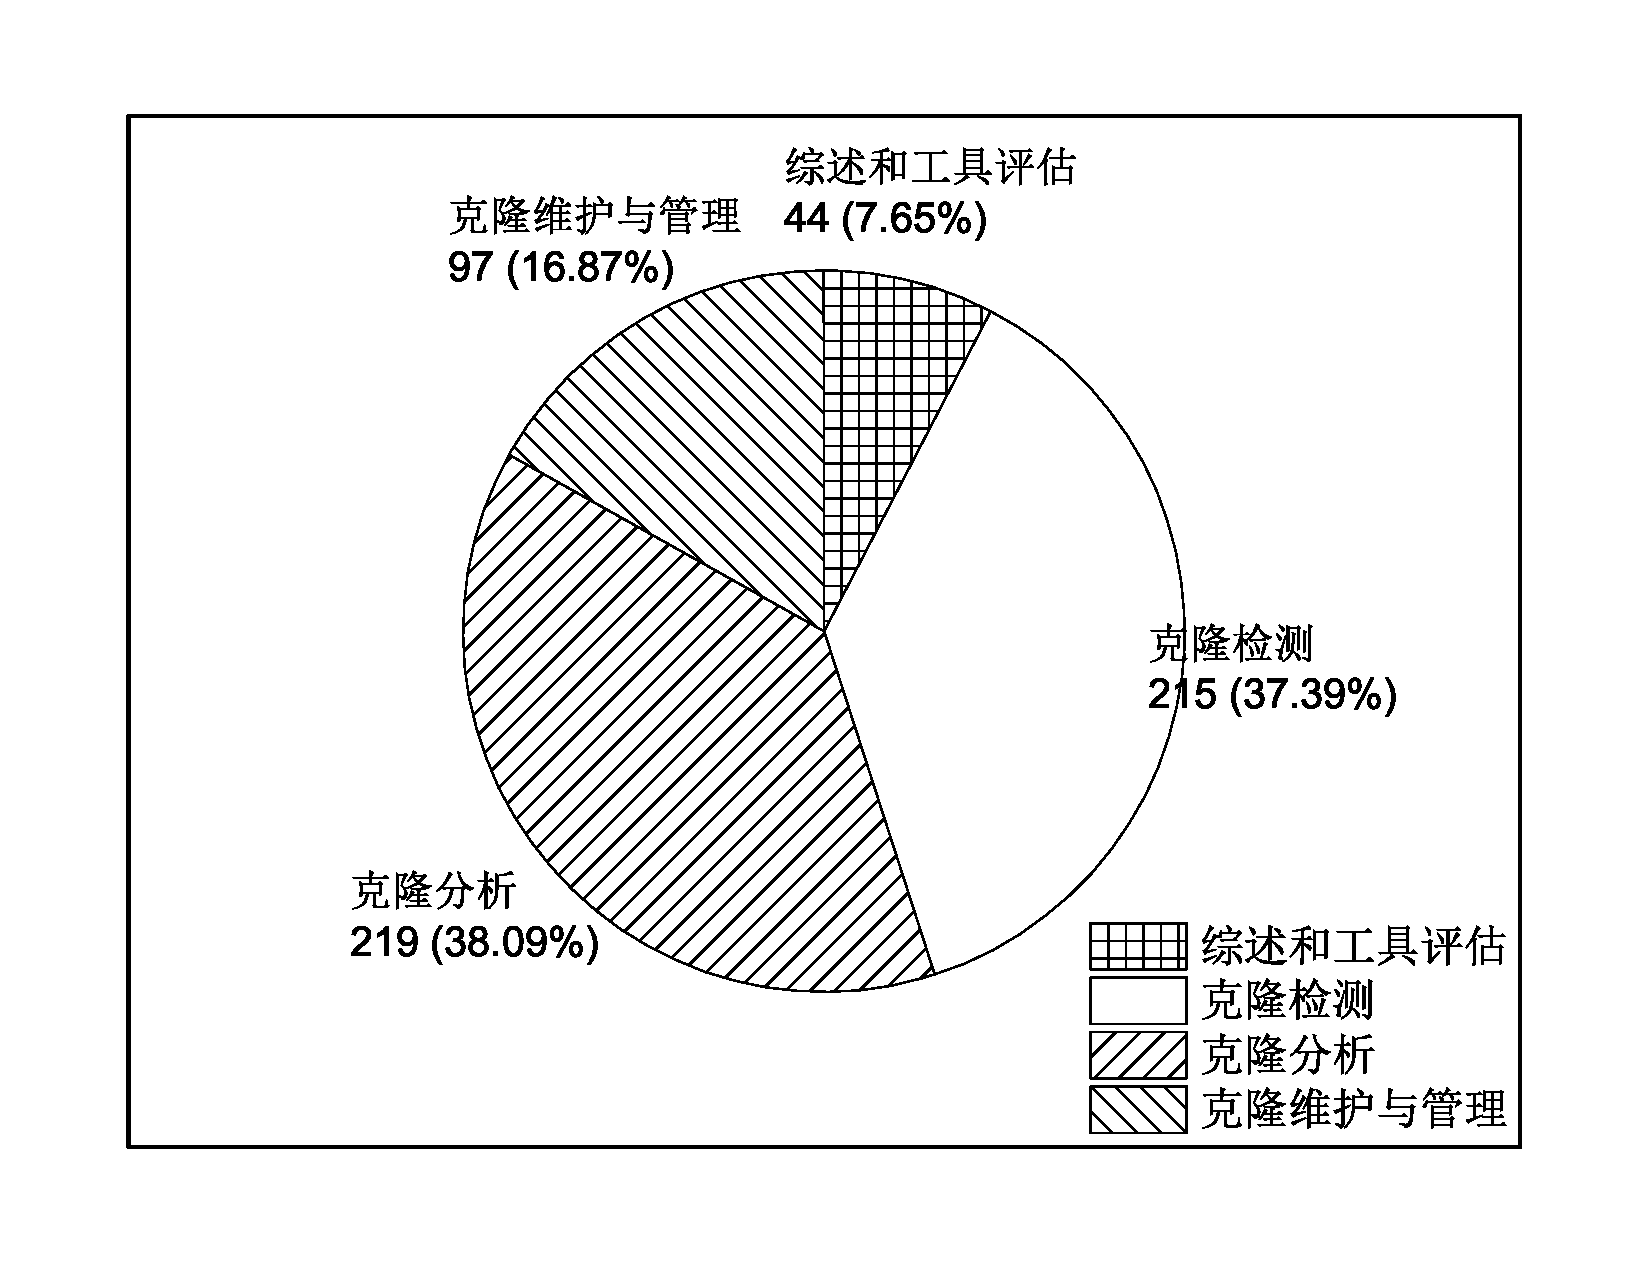
\includegraphics[width = 0.8\textwidth]{literaturedistribution1}
\bicaption[literaturedistribution1]{}{克隆代码研究领域文献分布}
{Fig.$\!$}{Literature distribution of code clone research}
%{Fig.$\!$}{Literature Distribution of Code Clone Research}
\vspace{-1em}
\end{figure}

根据此文献库中所给出的论文,Roy按照其分类进行了统计分析,分析了每个研究方向的论文分布情况和研究进展\cite{roy2014vision}。但是该文献库仅收录了2013年以前的文献,为了分析和反映克隆代码研究的最新进展、研究热点和发展趋势,本文在该文献库的基础上做了进一步的扩展,检索和收集了近几年的克隆代码相关文献,并按该文献库分类方式进行了重新统计和分析。本文统计和收集的文献共分为三类,即软件工程领域的重要国际会议论文、重要国际期刊论文以及相关学位论文。其中,重要国际会议论文为432篇,期刊论文113篇,学位论文30篇,共计575篇\footnote{本文统计的所有文献可分为两个部分:一是来源于阿拉巴马大学的文献库,二是笔者在进行研究期间所阅读整理和收集的文献。在收集的过程中,已经对文献进行了初步筛选,仅选取了领域内权威期刊、会议以及学位论文。} 。

克隆代码研究领域的文献统计分析结果如图~\ref{literaturedistribution1}~所示。从图中可以看出,目前研究中对克隆检测与分析的研究较为充分,是克隆研究领域的研究热点问题,分别占比37.39\%和38.09\%;而克隆维护与管理的研究论文占比较少(占16.87\%),说明目前对该方向的研究还方兴未艾。克隆综述和工具评估方面的研究占比更少,仅为7.65\%,说明目前较为实用的工具还不够充分。

\begin{figure}[htbp]
\centering
\includegraphics[width = 0.8\textwidth]{literaturedistribution2}
\bicaption[literaturedistribution2]{}{克隆领域每年发表的论文数量}
{Fig.$\!$}{Annual number of published papers of code clone research}
{Fig.$\!$}{Annual Number of Published Papers of Code Clone Research}
\vspace{-1em}
\end{figure}

\begin{figure}[htbp]
\centering
\includegraphics[width = 0.8\textwidth]{literaturedistribution3}
\bicaption[literaturedistribution3]{}{各个克隆研究活动每年发表的文献数量}
{Fig.$\!$}{Annual number of published papers of each clone research activity}
%{Fig.$\!$}{Annual Number of Published Papers of Each Clone Research Activity\vspace{-1em}
\end{figure}


为便于分析克隆代码研究领域的发展趋势,本文又对克隆代码研究领域的文献按照发表年份和研究方向进行了统计。统计分析结果如图~\ref{literaturedistribution2}~和~\ref{literaturedistribution3}~所示,其中图~\ref{literaturedistribution2}~是领域整体上每年发表文献数量的统计情况,图~\ref{literaturedistribution3}~是在不同研究方向上每年发表文献数量的统计情况。

从图~\ref{literaturedistribution2}~可以看出,克隆研究可以划分为两个阶段:1990-2003年和2004-2016年。在2003年以前,克隆代码研究领域的文献数量较少,这一阶段是克隆代码研究的孕育期。而在2004年以后的近10年内,克隆代码研究领域的文献数量快速增长,并且保持在一个较高的水平上,展现出了蓬勃的发展趋势,表明此阶段是克隆代码研究的发展期。与图~\ref{literaturedistribution2}~类似,从图~\ref{literaturedistribution3}~在不同研究方向上每年发表的文献数量来看,其研究趋势也以2003年为界限划分为两个阶段。在2003年以前,克隆代码研究主要集中在克隆检测方向,处于孕育期。在2004年以后,各个研究方向的文献数量都有了快速增长,进入了发展期。其中尤以克隆检测和分析方向的发展最为迅速,发表了大量研究成果,并依然有继续增长的趋势,说明克隆检测和分析事目前研究最为充分和最为活跃的研究方向。相比之下,克隆维护和管理仅在近几年才引起人们的关注,对克隆维护和管理的研究虽然近几年才刚开始起步,文献数量占比相对较少,但已呈现出逐年增长和后来者居上的趋势,说明克隆维护和管理正在逐渐成为克隆代码研究领域的新热点。

%\begin{figure}[htbp]
%\centering
%\subfigure{\label{literaturedistribution21}}\addtocounter{subfigure}{-2}
%\subfigure[Clone number of papers published each year in the field]{\subfigure[克隆领域每年发表的论文数量]{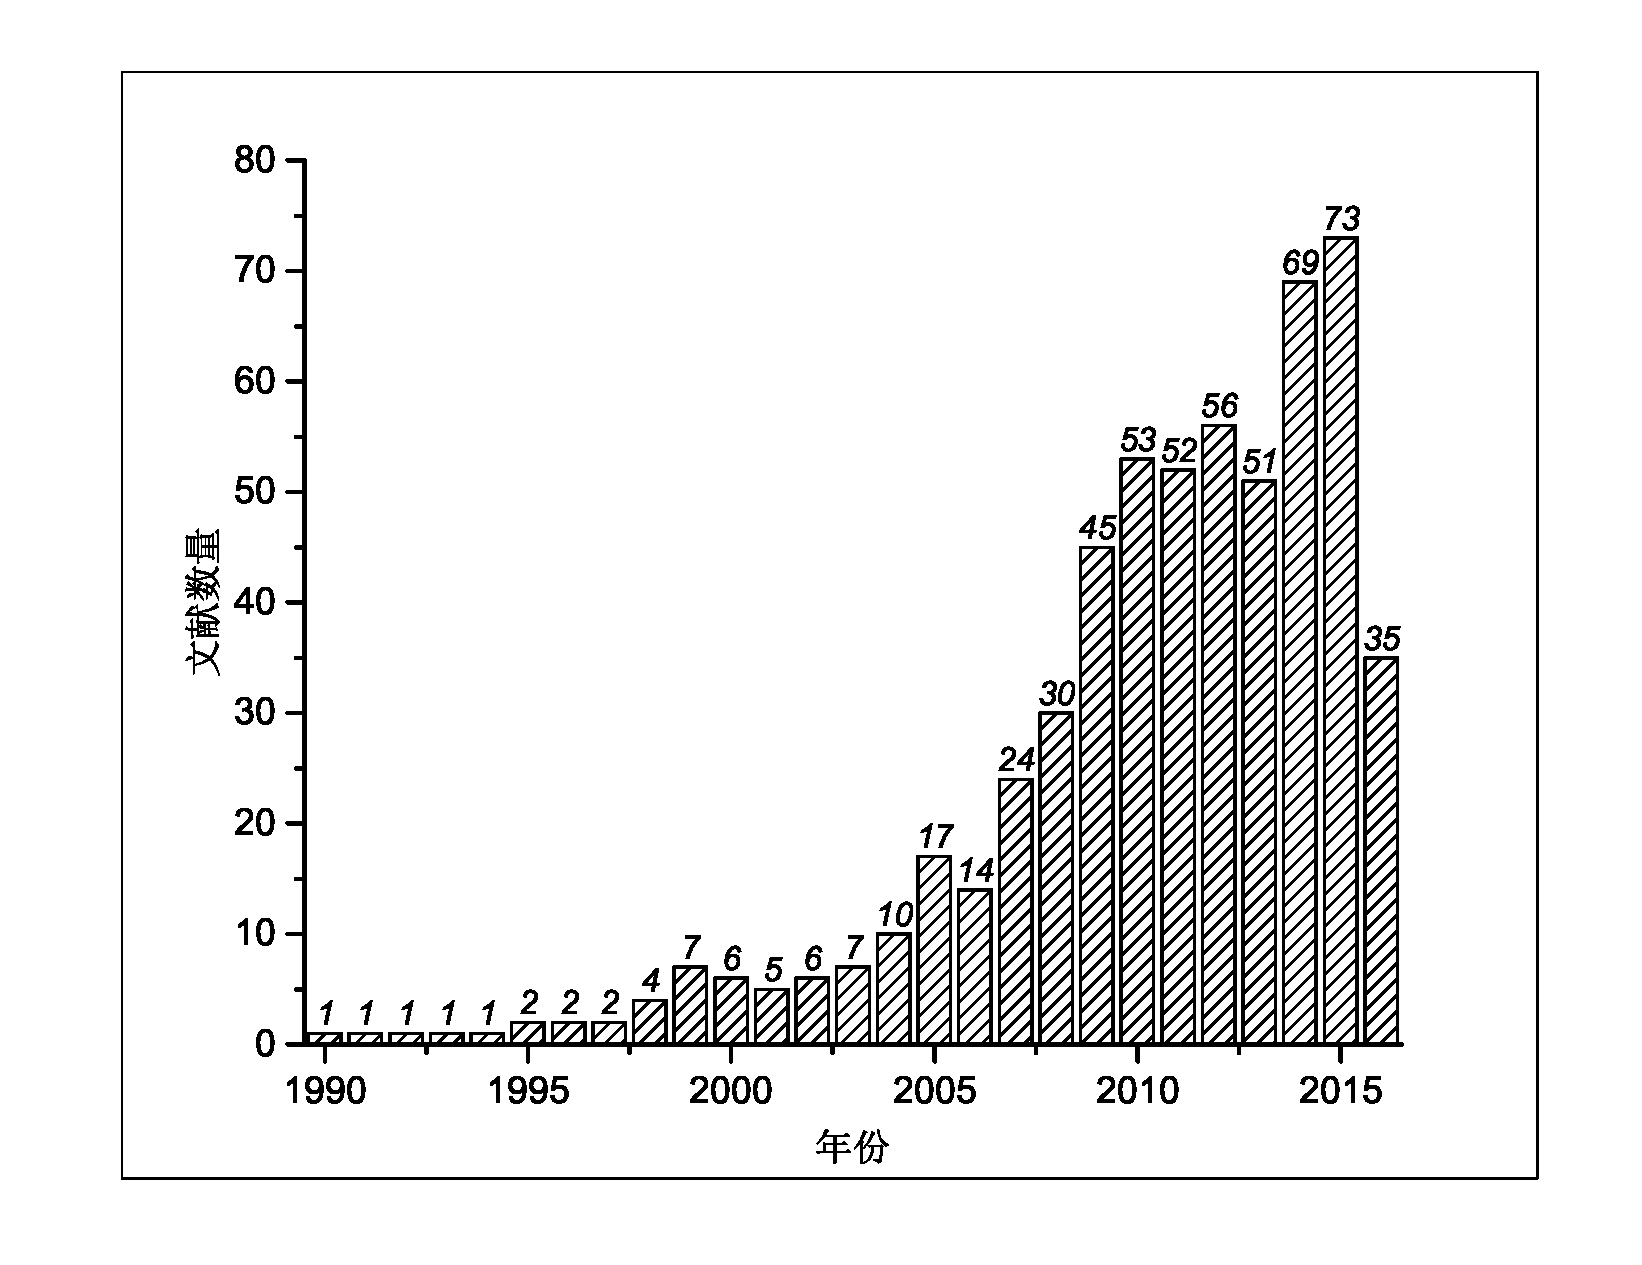
\includegraphics[width=0.8\textwidth]{literaturedistribution21}}}
%\subfigure{\label{literaturedistribution22}}\addtocounter{subfigure}{-2}
%\subfigure[Each clone number of events annually published literature]{\subfigure[各个克隆活动每年发表的文献数量]{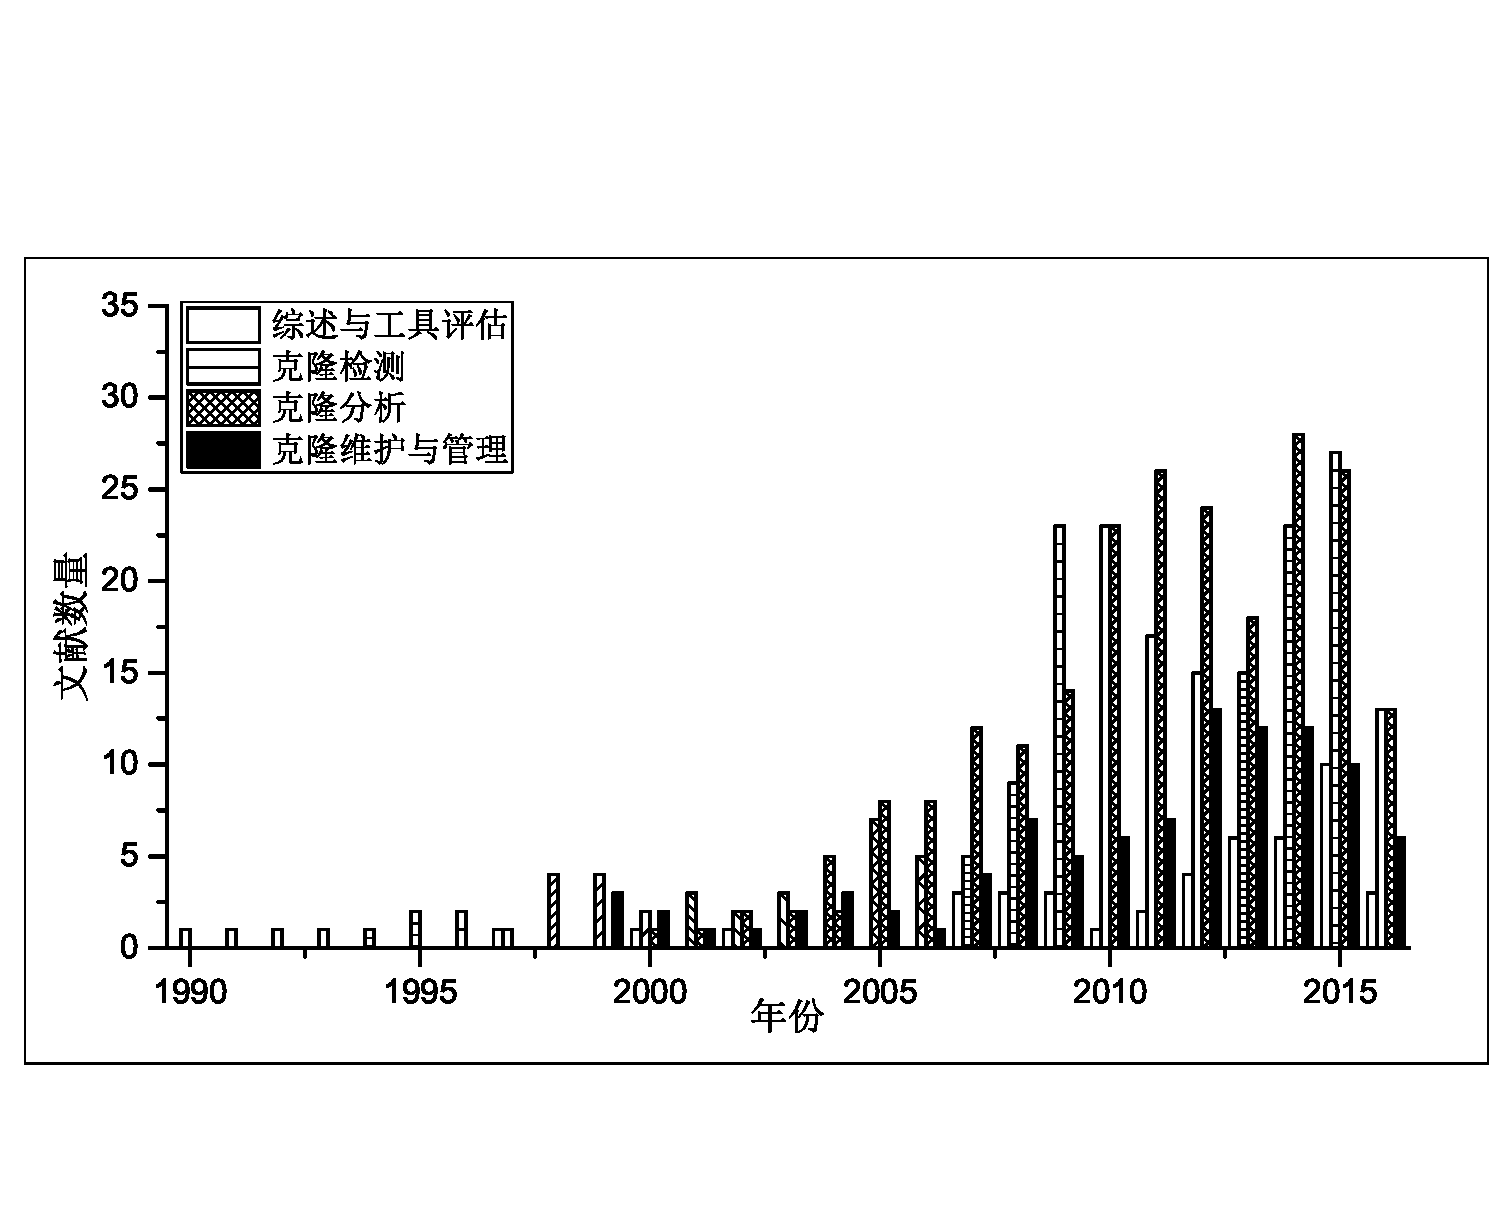
\includegraphics[width=0.8\textwidth]{literaturedistribution22}}}
%\bicaption[literaturedistribution2]{}{克隆代码领域研究趋势}{Fig.$\!$}{Cloning research trends in the code field}\vspace{-1em}
%\end{figure}

%为便于分析克隆代码研究领域的发展趋势,本文又对克隆代码研究领域的文献按照发表年份和研究方向进行了统计。统计分析结果如图~\ref{literaturedistribution2}~所示,其中图~\ref{literaturedistribution21}~是领域整体上每年发表文献数量的统计情况,图~\ref{literaturedistribution22}~是在不同研究方向上每年发表文献数量的统计情况。
%从图~\ref{literaturedistribution21}~可以看出,克隆研究可以划分为两个阶段:1990-2003年和2004-2016年。在2003年以前,克隆代码研究领域的文献数量较少,这一阶段是克隆代码研究的孕育期。而在2004年以后的近10年内,克隆代码研究领域的文献数量快速增长,并且保持在一个较高的水平上,展现出了蓬勃的发展趋势,表明此阶段是克隆代码研究的发展期。与图~\ref{literaturedistribution21}~类似,从图~\ref{literaturedistribution22}~在不同研究方向上每年发表的文献数量来看,其研究趋势也以2003年为界限划分为两个阶段。在2003年以前,克隆代码研究主要集中在克隆检测方向,处于孕育期。在2004年以后,各个研究方向的文献数量都有了快速增长,进入了发展期。其中尤以克隆检测和分析方向的发展最为迅速,发表了大量研究成果,并依然有继续增长的趋势,说明克隆检测和分析事目前研究最为充分和最为活跃的研究方向。相比之下,克隆维护和管理仅在近几年才引起人们的关注,对克隆维护和管理的研究虽然近几年才刚开始起步,文献数量占比相对较少,但已呈现出逐年增长和后来者居上的趋势,说明克隆维护和管理正在逐渐成为克隆代码研究领域的新热点。

\BiSubsection{克隆代码检测}
{Code Clone Detection }
\label{clonedetection}
克隆检测是指从软件中检测并报告克隆代码的位置的研究。相对于克隆代码研究的其他技术而言,克隆检测技术相对成熟。

\BiSubsubsection{克隆检测方法}
{Clone Detection Methods}

%%一般而言,克隆代码检测分为三个步骤:代码的中间表示、相似性匹配和报告检测结果。首先使用不同的方法对源代码进行抽象表示或转换,将其表示为抽象语法树等中间表示形式。然后对代码的中间表示形式进行相似性匹配,寻找相似的代码片段。最后报告检测结果,将彼此相似的克隆代码以克隆组的形式保存在检测结果中。
迄今为止,研究人员已提出许多种克隆检测方法,并开发了相应的检测工具。根据所使用的技术不同,可以将克隆检测划分为基于文本(Text)的方法、基于Token的方法、基于树(如Abstract Syntax Tree,AST)的方法、基于程序依赖图(Program Dependency Graph, PDG)的方法和基于度量值(Metric)的方法。

基于Text的克隆检测方法是通过直接比较源代码文本,使用字符串匹配等算法来检测克隆代码。因其并没有对源程序进行词法分析,大部分仅可以较好地支持Type 1克隆的检测。目前使用较多的基于文本的克隆检测工具主要有duploc\cite{ducasse1999language}、Simian\cite{Simian}、DuDe\cite{wettel2005archeology}、SDD\cite{lee2005sdd}、NiCad\cite{roy2008nicad}等。

基于Token的克隆检测方法是通过对源代码进行词法分析,获得源代码的Token序列,然后通过寻找Token序列中相似的子序列来检测克隆代码。因其对源代码进行了词法分析,所以可以较好地检测Type-2克隆代码的检测。但由于缺乏必要的语法和语义分析,使其无法较好地支持Type-3和Type-4克隆的检测。
目前使用较多的基于Token的克隆检测工具主要有Dup\cite{baker1995finding}、CCFinder\cite{kamiya2002ccfinder}、CP-Miner\cite{li2006cp}、iClone\cite{gode2009incremental}等。

基于Tree的克隆检测方法是将源代码表示为某种树的形式(如抽象语法树、代码解析树等),然后通过使用子树匹配算法从中寻找相似的子树来检测克隆代码。因其对源代码进行了语法分析,所以提高了克隆代码检测的准确率,尤其是可以较好地支持Type-3克隆的检测。但是由于子树匹配算法的时间复杂度高于前两种方法,因此这类算法的检测速度低于前两种方法。
目前使用较多的基于Tree的克隆检测工具有CloneDr\cite{baxter1998clone}、SimScan\cite{SimScan}、Deckard\cite{jiang2007deckard}、CloneDigger\cite{bulychev2008duplicate}等。

前三种克隆检测方法中所使用的中间表示形式较为容易实现,可使用程序静态分析方法或者编译器前端获得源代码的中间表示。大部分的克隆检测方法和检测工具属于前三种方法中的一种,可以检测系统中的大部分克隆代码。

基于PDG的克隆检测方法的主要思路是,将源代码转化成程序依赖图(包括数据依赖图和控制依赖图),然后通过寻找同构的子图来检测克隆代码。因程序依赖图表示了程序的语义信息,所以该方法可以支持语义相似的Type-4克隆代码的检测。但由于程序依赖图生成算法和图匹配算法的时间和空间复杂度极高,因而导致这类检测算法的时空开销过大,使其无法应用于大规模程序的克隆代码检测。
目前基于PDG的克隆检测工具主要有Duplix\cite{krinke2001identifying}等。

基于Metric的克隆检测方法是先将源代码转换为某种中间表示,然后在其基础上提取度量值并抽象为一个特征向量,然后通过计算特征向量的相似度来检测克隆代码。该方法的主要优点是检测速度快。但因基于度量值的方法高度依赖于度量值的提取,在对源码提取度量值的过程中会损失源码的部分语义信息,因此检测效果不够理想,使其应用受限。

此外,还有人使用结合两种或两种以上检测技术的混合方法来检测克隆代码。例如,Deckard在生成抽象语法树的基础上提取结构特征向量表示代码,然后使用聚类的方法寻找克隆代码\cite{jiang2007deckard}。CloneMiner先将源代码表示为Token形式,然后在此基础上通过使用频繁模式挖掘算法寻找相似模式来检测克隆代码\cite{basit2009data}。


\BiSubsubsection{克隆检测方法及工具评估}
{The Evaluation for Code Clone Detection Methods and Tools}

不同的克隆检测方法和检测工具各有其优缺点,分别适合检测不同类型的克隆代码,对同一类型的克隆代码的检测效果也不尽相同。如何针对具体的应用,选择合适的克隆检测方法和工具是困扰开发人员的一个问题。因此,
研究人员对主流的克隆检测方法及其检测工具进行了评估研究,以期为用户选择方法和工具提供指导性的建议\cite{bellon2007comparison}\cite{rattan2013software}\cite{roy2009comparison}\cite{svajlenko2014evaluating}。%%Bellon对6个克隆检测工具进行了评估,分别对比了查准率、查全率以及时间和空间等性能\cite{bellon2007comparison}。Rattan通过使用一种标准的系统文献综述方法,详细分析了克隆检测方面的213篇文献,并对不同的检测方法进行了评估分析,并给出了未来的研究方向\cite{rattan2013software}。此外,Roy重点分析了检测工具的使用技术和适用环境,对克隆检测工具的检测效果进行了详细的对比,对帮助用户选择和使用克隆检测工具有重要的指导意义\cite{roy2009comparison}\cite{svajlenko2014evaluating}。
本文也对目前较为主流的克隆检测工具和方法支持的克隆类型和检测效果等进行了评估,评估结果如表~\ref{detectionevaluation}~所示。其中,检测效果采用“较好”、“一般”和“较差”三种级别来评估:“较好”是指可以较好地支持该类型克隆代码;“一般”是指可以支持检测该类型克隆代码,但效果不佳;“较差”是指可以检测少部分的该类型克隆代码;对未支持的克隆类型未列出。

\begin{table}[htbp]
\bicaption[detectionevaluation]{}{主流克隆检测方法与工具评估}
{Table$\!$}{Evaluation for popular clone detection methods and tools}
\vspace{0.5em}
\centering
\wuhao
\begin{tabular}{cccc}
\toprule[1.5pt]
类型&工具或方法名&支持的克隆类型&检测效果\\
\midrule[1pt]
\multirow{5}{*}{Text} 
& Duploc\cite{ducasse1999language}&1、3&较好1,一般3\\
&Simian\cite{Simian}&1、2	&较好1,一般2\\
&DuDe\cite{wettel2005archeology}&1、3	&较好1,一般3\\
&SDD\cite{lee2005sdd}&1、3	&较好1,一般3\\
&NiCad\cite{roy2008nicad}&	1、2、3	&较好1、2、3\\
\hline
\multirow{4}{*}{Token} 
&Dup\cite{baker1995finding}&	1、2&较好1、2\\
&CCFinder\cite{kamiya2002ccfinder}&1、2&较好1、2\\
&CP-Miner\cite{li2006cp}&1、2、3&较好1、2,一般3\\
&iClone\cite{gode2009incremental}&1、2	&较好1,2\\
\hline
\multirow{4}{*}{Tree} 
&CloneDr\cite{baxter1998clone}&	1、2、3	&较好1、3,一般2\\
&SimScan\cite{SimScan}&	1、2	&较好1、2\\
&Deckard\cite{jiang2007deckard}&	1、2、3	&较好1、2,一般3\\
&CloneDigger\cite{bulychev2008duplicate}&	1、2、3	&较好1、3,一般2\\
\hline
\multirow{2}{*}{PDG} 
&Duplix\cite{krinke2001identifying}&	1、2、3、4	&较好1、2,一般3,较差4\\
&Gabel\cite{gabel2008scalable}&1、2、3、4	&较好1、2、3,一般4\\
\hline
\multirow{2}{*}{Metric} 
&Kontogiannis\cite{kontogiannis1996pattern}&	1、2、3、4	&较好1、2,较差3、4\\
&Mayrand\cite{mayrand1996experiment}&	1、2、3、4	&较好1、2,较差3、4\\
\bottomrule[1.5pt]
\end{tabular}
\end{table}

从表~\ref{clonedetection}~可以看出,基于Text的检测工具不支持Type-4克隆的检测。对Type-1克隆的检测效果最好,对Type-3克隆的检测效果一般。而对Type-2克隆支持较弱,仅有两个工具可以支持。原因是Type-2克隆是标识符重命名的克隆代码,基于Text的方法不能很好地处理标识符重命名问题。基于Token的检测工具同样不支持Type-4克隆的检测,但是可以较好地检测Type-1和Type-2克隆。支持Type-2克隆检测的原因是在将源程序转换成Token序列时进行了词法分析,因此可以解决标识符重命名的问题。但仅有一个工具可以检测Type-3克隆代码,并且检测效果一般。基于Tree的检测工具,同样不支持Type-4克隆的检测,但是对Type-1克隆的检测效果较好,并且几乎都支持Type-2和Type-3克隆的检测。由于采用的匹配算法不同,对Type-3即近似克隆的检测效果不尽相同,有些可以较好地支持Type-2克隆的检测,有些则较好地支持Type 3克隆的检测。基于PDG的检测方法不仅可以较好地检测Type-1和Type-2克隆,还可以以不同的程度支持Type-3和Type-4克隆的检测。但因其复杂度相对较高,使其并没有太多的检测工具可以利用。基于Metric的检测方法目前仅有一些检测方法被提出\cite{kontogiannis1996pattern}\cite{mayrand1996experiment},缺少相应的检测工具。

%可见,目前克隆检测方法对Type-1和Type-2克隆的检测最简单,因此效果最好,检测工具也最多;对Type-3克隆的检测相对于前两种有一定的难度,因此效果一般,但也有少量工具支持;对Type-4克隆的检测难度最大,因此效果最差,工具最少。此外,基于Text、基于Token、基于Tree的克隆检测方法实现容易,是目前较为主流的方法,相应的检测工具也较多。基于PDG的克隆检测方法受到图匹配算法复杂性的影响使得这类方法的实现难度较大,因此实用工具不多。而基于Metric的克隆检测因为检测效果不够理想,所以研究较少,也没有可用的检测工具。其次,目前绝大多数的克隆检测工具仅支持单版本的克隆代码检测,无法同时检测多个版本中的克隆代码。少数的克隆检测工具(如iClone)采用了增量式的克隆代码检测方法,即在旧版本克隆检测的基础上对新版本进行克隆代码检测,从而节约了检测时间,提高了检测效率。此外,目前绝大部分的克隆检测工具也没有集成到软件开发环境中,开发人员无法在开发过程中实时地检测和跟踪克隆代码。因此,研究如何提高Type-3和Type-4克隆的检测效果,以及如何在软件开发过程中增量式地检测克隆代码,这既是一个难点问题,也是未来的一个研究重点问题。

\BiSubsection{克隆代码分析}
{Code Clone Analysis}

克隆分析是指使用各种技术手段分析系统中的克隆代码,并挖掘其隐含的特征,旨在帮助软件开发人员更好地理解和维护克隆代码。目前的克隆分析研究主要集中在克隆演化分析、克隆评价分析上。

\BiSubsubsection{克隆代码演化}
{Code Clone Evolution}

%克隆代码往往存在于软件系统的多个版本中,并随着软件系统进行演化。
克隆代码演化分析就是通过分析克隆代码的演化过程,提取克隆代码的演化特征,识别克隆代码的演化规律,从而辅助人们更好地理解和维护克隆代码。克隆演化研究包括克隆演化过程分析和演化特征分析两个方面。演化过程分析即模型化克隆代码的演化过程。演化特征分析是分析克隆代码在演化过程中表现出来的演化特征或演化模式及其对软件质量的影响。

克隆演化过程分析最早是2001年由Antoniol等人提出的,使用时间序列描述克隆代码的演化模型\cite{antoniol2001modeling},但并未引起人们的重视。2005年,Kim提出了克隆家系模型用于描述克隆代码的演化过程,被认为是迄今为止最好的演化模型\cite{kim2005empirical}。Roy使用函数映射帮助构建克隆家系,并开发了gCad克隆家系提取器,大大提升了构建克隆家系的时间效率\cite{saha2011automatic}。Bakota通过映射不同版本的克隆来分析克隆代码的演化过程,并使用克隆坏味(Clone Smell)帮助分析克隆代码对系统的影响\cite{bakota2011tracking}。Harder对现有的演化模型进行分析\cite{harder2009modeling},指出通过分析克隆演化特征可以帮助程序开发和维护人员理解和维护克隆代码。

究竟哪些演化特征能真实准确地反映克隆代码的规律?这是克隆演化分析的难点问题。因此目前对克隆演化分析的研究主要集中在研究确定提取克隆代码的哪些特征作为演化特征以及如何提取这些特征。目前,常用的克隆演化特征主要包括克隆寿命、克隆稳定性与一致性变化。

%克隆寿命是指克隆代码在系统中的存在时间。Kim研究发现克隆代码要比非克隆代码更加稳定,同时寿命也更长\cite{kim2005empirical};进一步对长寿命的克隆代码进行研究后,发现对克隆代码的修改会使得克隆代码的寿命变短\cite{cai2011empirical}。Krinke通过对比克隆和非克隆代码,也发现克隆代码比非克隆代码的寿命更长\cite{krinke2011cloned}。通过对精确克隆和近似克隆的演化分析,发现其在演化过程中所表现出来的共同特点是:尽管克隆代码比率会随着时间而逐渐降低,但克隆代码的存在时间往往都会超过一年\cite{bazrafshan2012evolution}。因此,克隆代码会长时间的存在于系统中,在其生存期间克隆代码往往会发生变化,其变化规律与具体的软件系统相关\cite{gode2009evolution}。

%克隆稳定性关注的是在克隆代码的生存期内是否发生变化。被研究者普遍认可的观点是寿命较长的克隆代码是稳定的\cite{krinke2008cloned}\cite{gode2011clone}\cite{harder2013cloned},不会对系统造成不利的影响,也不会增加系统的维护成本。但是在克隆代码是否比非克隆代码更稳定这个问题上还存在一定的分歧。例如Gode研究发现大部分克隆是稳定的,不会发生变化\cite{gode2011frequency}。而Rahman的研究却发现克隆代码比非克隆代码更容易发生变化,是不稳定的\cite{rahman2014change}。Mondal给出了更为细致的分析结果,即Type-1、Type-2克隆是不稳定的,Type-3克隆是稳定的;并且发现克隆代码比非克隆代码的变化更分散,Type-3克隆比Type-1和Type-2克隆的变化更分散\cite{mondal2012comparative}\cite{mondal2012dispersion}。%%由此可见,在克隆代码的稳定性特征方面尚未达成共识,仍需要进一步研究。

%克隆代码的变化包括一致性变化和不一致性变化。遗忘一致性变化将会引发相关的软件缺陷,因此一致性变化也是克隆演化分析研究中需要关注的特征。Gode的研究发现发生一致性变化的克隆代码占克隆代码的比例很小\cite{gode2011frequency}。Krinke的研究进一步发现发生一致性变化和不一致性变化的克隆代码比例大约各占一半,并且大部分发生不一致性变化的克隆代码在后续的演化过程中不会继续发生变化\cite{krinke2007study}。Mondal等人的研究发现发生一致性变化的克隆代码可能会导致延迟传播现象。延迟传播是指某一个克隆片段的变化没有立即传播到其所在的克隆组中,而在间隔一定数量的版本后传播,继续发生一致性变化。研究表明延迟传播在Type-3的克隆中出现的更为频繁,软件开发人员应该重点关注Type-3克隆代码的变化,以避免引入克隆代码相关的软件缺陷\cite{mondal2016comparative}。

表~\ref{characteristic}~列出了目前对克隆演化特征的研究情况。由表中可以看出,研究者较为关注的克隆演化特征是克隆寿命、克隆稳定性与一致性变化。上述三个特征并不是相互独立的,克隆寿命会受到稳定性和克隆变化的影响,同时克隆稳定性与克隆变化之间存在对立关系。对克隆演化分析的研究大多属于实证研究,往往会较多地依赖于具体被用于实验分析的软件系统,这就导致了不同的研究可能得出不同的结论。例如对克隆稳定性的研究就出现了截然相反的观点。尽管如此,克隆演化特征分析依然可以给开发人员提供有价值的建议。一个普遍的共识是在维护和管理克隆代码的过程中更应关注那些克隆寿命较短、稳定性较差、发生一致性变化的克隆代码。%%但克隆寿命、克隆稳定性和一致性变化之间究竟存在着怎样的关系,它们对软件质量究竟会产生怎样的影响,还有哪些影响软件质量的克隆代码特征,还有待进一步深入的研究。

\begin{table}[htbp]
\centering
\bicaption[characteristic]{}{克隆演化特征分析}
{Table$\!$}{The analysis of clone evolutionary characteristic}
\vspace{0.5em}
\wuhao
\begin{tabularx}{0.9\textwidth}{llX}
\toprule[1.5pt]
文献&克隆模式、特征&结论\\
\midrule[1pt]
\cite{kim2005empirical}&	克隆寿命/一致性变化	&观察并分析克隆家系寿命与一致性变化规律\\
\cite{cai2011empirical}&	克隆寿命&	克隆寿命与克隆修改次数、新增和减少有关\\
\cite{krinke2011cloned}&	克隆寿命&	克隆代码的寿命比非克隆的寿命更长\\
\cite{bazrafshan2012evolution}\cite{gode2009evolution}&	克隆比率/寿命/变化规律	&克隆比率会随时间降低,会存在超过一年,存在期间变化规律往往和具体系统相关\\
\hline
\cite{krinke2008cloned}&克隆稳定性&	克隆代码比非克隆代码更稳定\\
\cite{gode2011clone}\cite{harder2013cloned}&	克隆稳定性&	克隆代码十分的稳定\\
\cite{gode2011frequency}&	克隆变化/一致性变化&	大部分克隆不会变化,一致性变化会更少\\
\cite{rahman2014change}&	克隆稳定性&	克隆会比非克隆更容易发生变化\\
\cite{mondal2012comparative}\cite{mondal2012dispersion}&	克隆稳定性/变化分布&	Type-1、Type-2是不稳定的,Type-3是稳定的;发现克隆代码变化比非克隆更加分散,同时Type-3克隆比Type-1和Type-2更加分散\\
\hline
\cite{krinke2007study}&	一致性变化&	一半的变化是不一致变化,且发生不一致性变化后,在后续的时间内会保持这种变化\\
\cite{mondal2016comparative}&	延后传播&	Type-3更容易发生延后传播并导致缺陷\\
\bottomrule[1.5pt]
\end{tabularx}
\end{table}


\BiSubsubsection{克隆代码评价}
{Code Clone Evaluation}

克隆评价分析主要是分析克隆代码对系统产生的影响,以便辅助开发人员更好地理解和维护克隆代码。克隆代码是否有害一直是克隆评价关注的一个热点,也是争论的一个焦点问题。因此,克隆评价研究主要是围绕着克隆代码是否有害而展开的,只是在不同阶段,人们对克隆代码的态度有所不同,研究的关注点也因此有所不同而已。

在研究的初始阶段,人们大多倾向于认为克隆代码都是有害的,因而研究的侧重点是克隆代码是否会引发软件缺陷(即克隆代码相关的缺陷分析),以及克隆代码是否会增大系统的维护代价(即克隆代码的维护代价分析)。然而随着对克隆代码研究的深入,人们研究发现虽然克隆代码有时会对软件质量产生一些负面影响,但并不一定都是有害的,从而引发了对克隆代码有害性的讨论(即克隆代码的有害性分析)。因此,克隆评价主要包括克隆相关的缺陷分析、克隆维护代价分析、克隆有害性分析等。

%在早期,有人认为克隆代码是一种最刺鼻的代码坏味,是因为它有可能会引发相关缺陷。因此,人们研究的关注点主要集中在克隆代码的缺陷分析上。例如,Juergens等人研究发现克隆代码的不一致性变化会引发相应的软件缺陷,从而降低了软件质量\cite{juergens2009code}。Gauthier通过对克隆代码进行安全性分析,在开源软件Joomla和Moodle中发现了几个潜在的影响软件质量的安全漏洞和缺陷\cite{gauthier2013uncovering}。但也有另外一些证据表明克隆代码的不一致性变化并不一定会引发缺陷,因此不会对软件质量产生显著的影响。例如,Bettenburg对不一致性变化是否引发缺陷的研究发现,仅有极少数的不一致性变化会引发缺陷\cite{bettenburg2009empirical}。文献\cite{wagner2016relationship}的研究则表明Type 3克隆代码中大约有17\%的代码含有缺陷,并且Type 3克隆不容易发生不一致性变化。文献\cite{elish2015fault}通过对缺陷密度的分析发现,面向对象程序中的克隆类含有更少的缺陷,并且Type 3克隆含有的缺陷最少。因此有人将克隆代码研究应用到缺陷检测中,但没有直接证据证明克隆代码与缺陷密切相关\cite{lo2012active}\cite{kamei2011empirical}。%%因此,克隆缺陷分析并不能直接证明克隆代码是有害的。

%除了克隆相关的缺陷分析外,还可以从维护代价的角度去分析克隆代码对软件产生的影响。Harder通过实验发现克隆代码的存在并不会增加缺陷修复的时间,但是缺陷未被修复则可能导致维护代价的增加\cite{harder2012controlled}。Lozano通过研究克隆代码的可变性,也发现克隆代码的存在会增加软件维护的代价\cite{lozano2008assessing}。Juergens不仅认为克隆代码会增加维护代价,还提出了一个计算模型来计算克隆维护代价\cite{juergens2010much}。而Monden的研究则发现包含少量克隆代码的软件模块比不含克隆代码的软件模块更可靠,但含有大量克隆代码的软件模块则正相反,实验表明克隆代码与软件可靠性和维护代价有一定的关联,但这种关联关系并不十分明确\cite{monden2002software}。以上维护代价分析的研究表明克隆代码的存在有可能会增加软件的维护代价,但是如何定量地计算克隆代码引起的维护代价仍然是一个尚未解决的问题。

%%虽然缺陷分析和维护代价分析可用于评价克隆代码对软件产生的影响,但却不能作为评价克隆代码是否有害的直观证据。正因如此,近些年来,研究人员又展开了克隆代码有害性分析的研究。Kapser通过对比11种克隆模式在软件开发和维护过程中的优缺点,并在开源软件Apache和Gnumeric上进行实证研究,发现在Apache中大约有71\%的克隆代码被分类为有益克隆,对系统维护具有积极的影响,是一种合理的存在方式,因此人们应当正视在开发过程中克隆代码的长期存在\cite{kapser2006cloning}\cite{kapser2008cloning}。Kapser通过对Apache Web Server中的克隆代码进行分析,研究发现其中一个子系统中聚集了大量的克隆代码;该子系统的克隆代码增加了系统的功能性,对软件开发过程是有益的\cite{kapser2006supporting}。Selim使用风险模型判定克隆代码是否有害,研究结果发现克隆代码并不比非克隆代码具有更高的有害风险\cite{selim2010studying}。Wang提出利用贝叶斯网络对克隆代码进行有害性预测的方法\cite{wang2012can},该方法可用于辅助开发人员决定是否可以通过复制粘贴的方式引入新的克隆代码。Higo则提出一种提取有问题的克隆代码(有害克隆)的方法,该方法先对程序进行标准化,然后利用检测工具检测克隆代码,最后对检测到的克隆代码进行过滤、合并等操作来提取有问题的克隆代码,在Linux内核2.6.6上的实验结果表明只有少数克隆代码是有问题的克隆代码\cite{higo2009problematic}。Hordijk提出了一个结构化的证据模型分析克隆代码的有害性,研究结果表明只有少部分的证据证明克隆代码是有害的,并且仍需更多的研究去支撑这一结论\cite{hordijk2009harmfulness}。%%从上述对克隆代码有害性分析的结果不难得出结论,克隆代码并非都是有害的,但是究竟具有什么特征的克隆代码是有害的,还是一个有待深入研究的问题。

表~\ref{evaluation}~对克隆评价分析研究进行了分类统计,使用“积极”、“中立”和“消极”三种评价标准对现有的克隆评价分析方法进行了总结。“积极”是指克隆代码的存在对系统有积极的影响;“中立”是指克隆代码不会对系统产生影响;“消极”是指克隆代码会对系统产生消极的影响。从表中可以看出,大部分研究对克隆代码持积极和中立的态度,仅有少数持消极态度。这从另外一个侧面表明目前对克隆代码是否有害还存在一定的分歧,主要原因是对克隆代码缺少统一的评价标准以及深入的特征挖掘与分析。%%,当然这也是克隆评价分析中的最具挑战性的问题。

\begin{table}[htbp]
\centering
\bicaption[evaluation]{}{克隆评价分析}{Table$\!$}{The analysis of clone evaluation}\vspace{0.5em}\wuhao
\begin{tabularx}{0.9\textwidth}{lllX}
\toprule[1.5pt]
&文献&评价&结论\\
\midrule[1pt]
\multirow{6}{*}{\rotatebox{270}{克隆缺陷分析}} 
&\cite{juergens2009code}&消极&研究发现不一致变化在克隆中发生较为频繁,同时也会导致相应的缺陷\\
&\cite{gauthier2013uncovering}&消极&通过对不安全的克隆代码分析,发现了几个安全漏洞和缺陷\\
&\cite{bettenburg2009empirical}&积极&克隆代码的不一致变化并不会引入缺陷,不会对软件的质量产生影响\\
&\cite{elish2015fault}&积极&克隆代码含有更少的缺陷,Type 3所含有的缺陷最少\\
&\cite{lo2012active}&中立&克隆代码研究应用到缺陷检测中,但没有直接证据证明与缺陷相关\\
&\cite{kamei2011empirical}&中立	&通过实验发现并不会增加缺陷修复时间,但是缺陷未被修复,可能会产生维护代价的增加\\
\midrule[1pt]
\multirow{4}{*}{\rotatebox{270}{克隆维护代价分析}} 
&\cite{wagner2016relationship}&中立	&Type 3克隆中有17\%含有缺陷,并且Type3克隆更容易发生一致性变化\\
&\cite{harder2012controlled}&消极&通过对克隆代码的可变性研究发现克隆代码确实会增加其方法可变化的维护代价,但没有确切的证明会说明克隆会增加系统维护代价\\
&\cite{juergens2010much}&消极&认为克隆会增加维护代价,并且提出了一个代价计算模型计算这次代价\\
&\cite{monden2002software}&中立&Monden却发现包含克隆的模块比不含克隆的模块更可靠,同时含有大量克隆的模块却相反实验表明了克隆与系统可靠性和维护代价的关系,但是这种关系仍然不够明朗\\
\midrule[1pt]
\multirow{6}{*}{\rotatebox{270}{克隆有害性分析}} 
&\cite{selim2010studying}&积极&克隆代码并不比非克隆代码具有更高的有害风险\\
&\cite{kapser2006cloning}\cite{kapser2008cloning}&积极	&发现最多有71\%的克隆对系统的可维护性具有积极的影响\\
&\cite{rahman2012clones}&积极	&克隆并不是真正的代码坏味,克隆是无害的\\
&\cite{wang2012can}&中立	&预测克隆有害性,其中有害的较少,无害的较多\\
&\cite{higo2009problematic}&中立&使用分类模型抽取有问题的克隆代码,只有少部分是有问题的克隆\\
&\cite{hordijk2009harmfulness}&中立&现有研究不能支撑克隆有害的观点,仍需进一步的研究\\
\bottomrule[1.5pt]
\end{tabularx}
\end{table}

\BiSubsection{克隆代码维护}
{Code Clone Maintenance}

克隆维护是解决克隆代码问题的直接途径,主动地解决克隆代码可能或已经引发的问题。克隆维护与软件开发过程结合得较为紧密,维护的方法主要包括克隆重构、克隆规避、克隆复用和克隆管理。

\BiSubsubsection{克隆代码重构}
{Code Clone Refactoring}

重构作为一种常见的软件维护手段,是指在不改变软件外部行为的条件下改变软件的既有设计\cite{kerievsky2006重构与模式}。重构应用于克隆维护中,指的是通过重构手段消除系统中的克隆代码。

由于重构所需的条件较为苛刻,同时重构的代价也较大,还需考虑重构安全的问题。因此,在重构前对克隆代码进行可重构性分析和重构排序显得尤为重要。可重构性分析旨在识别适于重构的克隆代码候选集合,以提高克隆重构的效率。Lin等人通过对克隆代码进行差异性分析,帮助开发人员决定是否进行重构操作和如何执行重构操作\cite{lin2014detecting}。Mende实现了一个工具支持可重构性分析,在软件中识别可以被重构的函数克隆\cite{mende2009evaluation};Schulze提出了一个用于识别可重构的克隆代码的克隆分类方法,通过计算克隆代码的可重构指数识别可重构的克隆代码\cite{schulze2008towards};Choi等人提出了基于度量值的可重构性分析方法,可以快速地识别可重构的克隆代码\cite{choi2011extracting}。识别可重构克隆后,为了节省重构时间,还可以对克隆代码进行重构排序或者调度。如Mandal先通过分析克隆演化模式来确定克隆候选,然后使用关联规则挖掘进行可重构排序、\cite{mandal2014automatic};Lee采用遗传算法对重构进行调度,以确定重构顺序帮助改进软件质量\cite{lee2011automated};Zibran提出一种极限编程方法对克隆代码进行重构调度\cite{zibran2011constraint}。另外,Liu等人提出了一个重构调度方法帮助优化调度过程\cite{liu2012schedule}。尽管该方法不是针对克隆重构的,但也可以考虑将其应用于克隆代码的重构调度上。此外,Radhika等人仅考虑重构代价对所有的克隆代码进行重构排序,未考虑克隆代码是否适合重构的问题\cite{venkatasubramanyam2013prioritizing},应该结合可重构性分析指导克隆重构。
克隆重构最主要的目的是消除系统中的克隆代码。Higo等人开发了一个工具ARIES,根据克隆代码的结构信息识别可重构的克隆代码,然后通过计算不同的度量值来确定使用哪一种目前已有的重构方法移除克隆代码\cite{higo2008metric}。Krishnan通过分析克隆代码的程序依赖图,确定给定克隆代码能否被安全的重构,然后通过检测和参数化克隆代码的差异点对克隆代码进行重构,取得了较好的效果\cite{krishnan2014unification}。Barbosa使用四种规则重构克隆代码,并在开源软件JhotDraw上进行了实验,结果表明基于规则的重构方法可以有效地移除软件中的克隆代码\cite{barbosa2013removing}。

在重构完成后,对重构后代码进行分析,还可以得出一些结论以进一步指导克隆重构。G{\"o}de通过对维护人员使用的重构方法和被重构的克隆代码进行实证研究,发现在不同的软件系统中都存在克隆重构的行为,并且克隆重构不是经常性地发生而是有选择性地发生\cite{gode2010clone}。Zibran等人通过克隆重构研究,回答了所提出的关于克隆重构的七个研究问题,并且研究发现克隆规模对克隆重构没有重要的影响,同时在软件早期的版本中重构会较为频繁地发生,发生重构的克隆在重构前往往是较为稳定的克隆代码\cite{zibran2013evaluating}。Choi通过对重构行为进行观测,识别出几种较为频繁的克隆重构模式,并且分析了每种重构模式的特征,这些都有助于进一步指导克隆代码的重构\cite{eunjong2014investigation}。Tairas通过对克隆代码的重构性分析,提出了子克隆的概念,并研究发现子克隆的重构行为更容易发生,因此建议在对克隆代码的维护过程中应重点考虑子克隆的重构\cite{tairas2010sub}。

%%目前,虽然已有重构方法以插件的形式集成到了eclipse中 ,支持在软件开发过程对一般代码坏味重构。由于一般代码坏味的重构方法不一定适合克隆代重构,所以尚未有在软件开发环境中针对克隆代码的重构方法。此外,重构是在克隆代码出现后用以消除克隆代码的一种被动的软件维护方法,而且并非所有的克隆代码都适合重构。因此重构不是解决克隆代码维护难题的最有效的方法,更有效的方法是在软件开发过程中主动地规避或维护克隆代码,这是克隆维护中的一个难点问题。

\BiSubsubsection{克隆代码规避}
{Code Clone Prevention}

克隆规避也称克隆预防,是在克隆产生时通过某种策略或手段进行干预,以避免克隆代码的产生。克隆规避是一种预防性的克隆维护方法,通过阻止克隆代码产生来降低克隆维护的代价。

软件开发人员的复制粘贴活动是导致克隆代码产生的最主要原因。因此在复制粘贴时对新产生的克隆代码进行分析,帮助软件开发人员决定是否规避克隆代码,是目前常见的克隆规避方法。Ali曾提出一个克隆规避的概念模型\cite{ali2013enhancing},尽管对克隆规避研究具有一定的指导意义,但并未给出该模型的具体实现方法。Wang等人基于贝叶斯网络在复制粘贴时预测克隆代码的一致性变化,通过判断一致性变化决定是否规避该新产生的克隆代码\cite{wang2012can}\cite{wang2014predicting}。Ravikanth通过分析复制粘贴操作的前置和后置条件,来确定是否允许对被复制的克隆代码实施粘贴操作,从而实现克隆规避\cite{venkatasubramanyam2012method}。

%%由于受软件复用的影响和编程语言的限制,大部分克隆代码是无法避免的。克隆规避可以作为一种辅助的手段通过限制开发人员在软件开发过程中的复制粘贴操作帮助减少克隆代码的产生,但却无法规避全部的克隆代码。在实际的应用中,还需要将克隆规避和克隆管理相结合,对可以规避的克隆代码采用规避技术进行主动地规避,对无法规避或者无需规避的克隆代码采用跟踪的方式进行管理,以主动地维护这些代码。

\BiSubsubsection{克隆代码复用}
{Code Clone Reuse}

在软件开发过程中,复用既有代码是一种常见的软件开发手段。近些年来,随着对克隆代码评价分析研究的深入,人们已经意识到复用健壮性好的克隆代码不仅有助于缩短软件开发周期,还有利于提高软件的健壮性和可维护性。%%因此,对克隆复用的研究在近些年来引起了人们的关注,成为克隆代码领域中的一个新的研究方向。不过,相对于克隆检测和分析而言,目前对克隆复用的研究还相对较少。

Krutz等人提出克隆数据库概念,将已有克隆代码组织为克隆数据库,并结合代码检索技术实现对克隆代码的复用\cite{krutz2014code}。Ishihara提出的方法也允许开发人员通过代码搜索技术搜索可以复用的克隆代码\cite{ishihara2013reusing}。Ohta通过对比软件开发过程中由复制粘贴操作产生的克隆代码和系统中已存在的克隆代码,并将该克隆代码划分为较差、较好、最好三种情况,辅助开发人员决定是否能够复用该克隆代码\cite{ohta2015source}。但该方法对克隆代码的可复用性评价仅依赖于开发人员的复制粘贴操作,仅在复制粘贴操作发生后给出可复用性建议,无法在复制粘贴操作发生前为开发人员提供可复用的克隆代码信息。在软件开发过程中直接向开发人员提供一个已经通过某种评价方式确定是否可复用的克隆代码库,是一种更为主动的克隆代码复用形式。例如,Yang\cite{yang2015classification}等人使用机器学习模型对克隆代码进行分类,分类标准由开发人员动态地标记,通过标记可复用的克隆代码将该方法应用于克隆复用,辅助开发人员搜索可以复用的克隆代码。Ohtani从代码建议的视角辅助开发人员复用已有的代码,从不同粒度(关键字级别、方法级别和混合方法)对可复用的代码提供搜索支持,实验结果表明混合方法可以更精确地提供代码是否可复用的建议\cite{ohtani2015level}。Kintab实现了一个克隆代码的专家推荐系统,可以在线向软件开发人员提供复用克隆代码的相关咨询,软件开发人员可以根据专家的建议决定如何复用和维护既有的克隆代码\cite{kintab2014recommending}。

%%软件复用在提高软件开发效率的同时,势必也导致产生大量的克隆代码,这就使得克隆复用研究面临着一些新的问题。例如,如何实时地跟踪、维护和管理一个可复用的克隆代码库,在保证软件开发质量的前提下,主动地复用既有代码,以提高软件开发效率,既是一个新问题,也是一个难点问题。

现有的克隆代码复用研究大都是针对单一项目的。如何实现对跨项目的克隆代码复用是克隆复用面临的另一个新问题。目前,在互联网环境下,大量的开源社区里也普遍存在代码复用的情况,由此产生了跨项目的克隆代码和对跨项目代码复用的应用需求。但目前对这种跨项目的克隆代码复用的研究依然较少。Ishihara对跨项目的软件进行函数克隆检测,试图建立一个公用函数库用于代码复用\cite{ishihara2012inter}。Cheng等人研究了跨项目的克隆代码检测技术\cite{cheng2016feasibility}。Tairas等人将信息检索技术与克隆代码分析相结合,以便快速有效地搜索可复用的克隆代码\cite{tairas2009information}。事实上,以上这些技术都可以用于跨项目的克隆代码搜索和复用中。

\BiSubsubsection{克隆代码管理}
{Code Clone Management}

%%克隆代码的重构是在克隆代码产生之后消除克隆代码及其对系统产生的影响,这种维护方式属于一种较为被动的维护方式,其维护代价本来就较高。而克隆代码往往又会随时间的推移和需求的变更而在软件系统中发生变化或者产生新的克隆代码,频繁地重构势必进一步增大克隆代码维护的代价。如果将克隆代码的维护提前到软件开发阶段,在软件开发过程中跟踪克隆代码的变化,并主动地规避克隆代码的产生,则势必会降低后期维护的代价。而若要实现这种主动的维护方式,则需要从克隆代码管理的角度解决克隆代码的维护难题,即通过在软件开发过程中实现边开发、边管理克隆代码,以主动的方式维护克隆代码,消除克隆代码对软件系统的不利影响。

克隆代码管理(简称克隆管理)的概念最早是1997年由Koschke提出的\cite{koschke2008frontiers},但当时并未引起人们的重视。随着克隆代码规模的逐渐增大,人们发现现有手段无法有效解决克隆代码维护难的问题时,才开始把目光重新转向对克隆管理的研究。目前克隆管理被认为是解决克隆代码维护难题的最有效的方式。早在2012年的面向工业界的克隆管理会议\footnote{Software Clone Management Towards Industrial Application}中,就有专家学者指出克隆管理是未来的重要研究方向,如何将克隆管理与软件开发过程相结合并使之适用于工业界是目前克隆研究领域急需解决的问题\cite{koschke2012software}。%%但是目前人们对克隆管理的研究仍处于起步和理论研究阶段,罕有从管理的角度维护克隆代码的研究报道。

%Koschke将克隆管理划分为预防性、补偿性和改正性三种类型\cite{koschke2008frontiers}。预防性克隆管理的目标是避免克隆代码,关注于避免新的克隆代码的产生,而不是对已有克隆代码的管理。补偿性克隆管理的目标是发现克隆代码所引发的问题,并对其对系统造成的不利影响进行补偿。改正性克隆管理的目标是以主动的方式消除可能对系统产生不利影响的克隆代码。然而,Koschke对克隆管理的这种划分方法的理论意义大于实际意义。目前克隆管理研究主要集中于补偿性克隆管理,而改正性克隆管理尚未具体应用到实际的克隆管理中。

%Roy在文献\cite{roy2014vision}中对克隆管理研究进行了详尽的阐述,指出目前对克隆管理的研究依然较少,尚缺少有效的克隆管理方法,尤其是对Type 3和Type 4克隆代码进行管理的研究还不够充分,未来应针对这两种类型的克隆代码的管理进行深入研究。尽管Roy对克隆管理的分析涵盖了克隆代码领域的大多数研究内容,但只是以工作流的形式组织这些研究内容,并未考虑这些研究内容之间的联系,彼此之间的信息是相互割裂的,同时也没有结合软件开发过程分析对克隆管理的要求,更没有给出具体的克隆管理方法。

克隆代码管理的主要目的是降低克隆代码维护的代价。目前克隆管理的研究内容主要包括克隆跟踪、克隆变化管理以及克隆管理工具。其中,克隆跟踪是研究跟踪克隆代码产生和变化的方法。克隆变化管理是研究对克隆代码的变化进行管理的方法。克隆管理工具是研究开发有效管理克隆代码的工具。

克隆管理需要解决的首要问题是如何实时地跟踪系统中的克隆代码,包括克隆代码的产生及其变化。由于复制粘贴操作是导致克隆产生的主要原因,因此对克隆跟踪的研究主要是通过监测程序员的复制粘贴操作来实现的。例如,许多克隆跟踪工具CLONEBOARD\cite{de2009managing}、CnP\cite{hou2009cnp}、CPC\cite{weckerle2008cpc}、CReN\cite{jablonski2007cren}、CSeR\cite{jacob2010actively}等都是在软件集成开发环境中跟踪克隆代码的产生,但并非都能跟踪克隆代码的变化。另一方面,在软件开发过程中克隆代码可能随时发生变化,因此要实现对克隆代码的管理,不仅要跟踪克隆代码的产生,还要跟踪克隆代码的变化。Duala使用克隆区域描述符描述生成克隆代码的上下文信息,然后根据这些上下文信息实时跟踪克隆代码的变化\cite{duala2008clonetracker}\cite{duala2010clone}。该方法仅通过实验验证可以跟踪克隆代码的变化,但是并没有实现可用的插件集成到集成开发环境中,以实现对克隆代码的边开发、边管理。

跟踪克隆代码的目的是为了对克隆代码进行维护和管理。为了实现边开发、边管理克隆代码,还要对克隆代码的变化进行维护和管理。Yamanaka等人\cite{yamanaka2013applying}将克隆变化与事件通知机制相结合,将每一个克隆变化都看成一个事件,在克隆发生变化时提醒开发人员及时地对克隆变化进行维护。Cheng等人\cite{cheng2016rule}提出了一个基于Token的克隆代码一致性维护方法,当克隆组内的一个代码发生变化时,能够同时修改组内的其他克隆代码,保证克隆代码的一致性。该方法的前提是已知克隆变化需要一致性维护,但没有给出克隆变化是否需要一致性维护的判定方法。因此,Zhang等人\cite{zhang2016predicting}在克隆代码发生变化时预测克隆代码一致性维护需求。该方法通过提取克隆代码的演化信息及其相关特征,在克隆代码发生变化时辅助开发人员确定克隆变化是否需要一致性维护。Mondal等人通过对克隆组内的克隆代码排序,从而预测需要一致性维护的克隆代码\cite{mondal2014prediction}。此外,Murakami等人在克隆代码未发生变化时,预测克隆代码的下一次变化\cite{murakami2014predicting}。该方法通过分析历史版本中的克隆代码的变化情况,提取相关的特征进行变化预测,以便在软件开发过程中提醒开发人员对有可能发生变化的克隆代码进行维护。可见,克隆变化管理的关键不仅需要实时跟踪克隆代码的变化,更重要的是对发生变化的克隆代码进行及时的维护。

前面的研究只是针对不同的侧重点提出的克隆管理方法,却没有提供可以实际应用的克隆管理工具。鉴于此,Zhang基于事件通知机制实现了一个克隆管理工具,不仅可以监测克隆代码的产生,还可以监测克隆代码的维护过程\cite{zhang2013towards}。Nguyen实现了一种可用于管理克隆代码的eclipse插件JSync\cite{nguyen2012clone}。该插件支持在软件开发过程中对克隆代码进行克隆关系管理与一致性维护管理。这里的克隆关系管理是指在软件开发过程中检测系统中的克隆代码,并对具有克隆关系的代码进行管理。这里的一致性维护管理是指识别变化的克隆代码以及变化的克隆代码是否会导致不一致性缺陷,以便开发人员对克隆代码进行一致性维护。而另一个较早提出的eclipse插件CeDAR\cite{tairas2012increasing}。虽然没有强调是一种克隆管理工具,但事实上也具有一定的克隆管理功能。该插件将克隆检测和克隆重构融为一体,对现有克隆检测工具的克隆检测结果进行可重构性分析,寻找潜在的可重构的克隆代码,然后在软件开发过程中实现对克隆代码的重构。

%%如何将克隆代码的检测、分析和维护结合到软件开发过程中,以实现对克隆代码的边开发、边维护和边管理是克隆管理急需解决的一个难点问题。

\BiSubsection{当前研究中存在的问题分析}
{Problems in Current Research}

克隆代码研究已经成为了软件工程领域的一个热点问题,目前的克隆研究已经取得了相当丰富的研究成果,如克隆检测、克隆分析和克隆维护研究等,但目前的研究中仍然存在一些问题。

(1)克隆检测研究可以帮助程序开发人员快速的获得系统中的克隆代码,是目前研究的较为深入且广泛的一个研究活动。已经开发和提出了相当规模的克隆检测方法和工具,使用其可以快速高效地检测系统中存在的克隆代码。但是,克隆代码检测仅仅是克隆研究的初始阶段,即不能帮助软件开发人员理解克隆代码,又不能解决克隆代码对软件产生的不利影响。因此,克隆代码分析和维护研究将是解决克隆代码问题的关键内容。

(2)克隆代码分析可以辅助开发人员理解克隆代码,也是目前克隆代码研究中最为活跃的一个分支。在克隆分析的研究中,克隆代码演化研究是最为重要的研究内容,克隆评价研究往往也是在克隆代码演化的基础上进行,尤其是体现在演化过程的克隆代码变化对软件的影响上。但是,克隆演化分析研究中仍然不能令人满意。首先最重要的是,在目前的克隆代码的演化研究中,研究人员的研究往往集中到某一个具体的克隆代码的演化特征上,缺少从宏观上的对克隆代码演化特征的分析。例如,研究人员分别研究了克隆代码的克隆寿命、稳定性等某一个具体的问题。其次,克隆演化研究也往往带有较强的主观性,研究人员往往是通过分析既有的系统验证固有的结论,甚至出现了完全不同的研究结论。例如在对克隆代码稳定性的研究中,有研究者认为克隆代码是稳定的,也有研究者认为非克隆代码是稳定的。因此,如何从大量的克隆代码及其演化过程中全面且客观地识别克隆代码的演化特征是一个值得研究的问题。克隆代码的演化特征对于帮助程序开发人员理解克隆代码及其演化过程具有积极的意义,可以进一步提高软件的可理解性。


(3)克隆维护研究旨帮助程序开发人员解决或者避免克隆代码对系统产生的不利影响的问题。在克隆维护研究中研究人员进行了大量的研究,包括对克隆代码的重构、复用和管理等等。然而,目前克隆维护研也不能令人满意。%首先,克隆重构作为消除克隆手段,但由于其重构条件苛刻,仅能消除一小部分克隆代码,维护代价偏高。同时,由于多种原因无法规避全部的克隆代码,也无法解决克隆代码的维护难题。此外也缺少成熟有效的复用模型和方法。更为重要的是,
上述克隆维护研究没有聚焦到导致克隆代码难以维护的根本原因上。克隆代码难于维护的根本原因在于克隆代码在其演化过程的中的变化问题,尤其是克隆代码的一致性变化和不一致变化,及其由此所引发的克隆一致性缺陷和额外的维护代价问题。%克隆代码的一致性维护问题是影响软件质量的一个重要因素。克隆代码的一致性变化问题可能会导致新的克隆缺陷,而保持这种一致性也会导致克隆代码的维护代价变大,因此研究克隆代码的一致性维护需求预测显得尤为重要
如何避免、解决克隆代码的一致性变化问题是克隆维护研究中的一个值得研究的问题。通过预测克隆代码的一致性维护需求,可以有效的避免一致性缺陷,也可以降低克隆代码所导致的代价,并进一步帮助提高软件质量和可维护性。

%克隆维护是处理克隆代码所引发的相关问题的直接途径,其主要任务是通过采取措施维护系统中的克隆代码。克隆重构作为消除克隆手段,但由于其重构条件苛刻,仅能消除一小部分克隆代码,并且克隆重构属于一种被动的维护方式,维护代价偏高。一种较为主动的维护方式是克隆规避,即通过监测复制粘贴活动从源头上避免有害克隆代码的产生。但由于多种原因无法规避全部的克隆代码,也无法解决克隆代码的维护难题。此外,克隆复用作为一种常用的可以帮助提高软件开发效率的手段,依然缺少成熟有效的复用模型和方法。最后,克隆重构和复用往往需要克隆分析结果的支持,如克隆评价结果指导克隆重构和克隆复用,然而遗憾的是目前的克隆维护没有与克隆分析相结合。

\BiSection{研究内容与论文结构}
{Main Research Contents and Structure of This Dissertation}

\BiSubsection{研究内容}
{Main Research Contents}

针对软件中所存在的大量的克隆代码、以及克隆在其演化过程容易被程序开发人员修改而导致克隆代码的一致性维护问题,本文结合程序分析、克隆演化和度量提取,研究基于机器学习的克隆代码演化分析与一致性维护方法,可以有效的帮助程序开发人员理解克隆代码,并可以降低克隆代码的维护代价和避免克隆一致性缺陷,以达到提高软件质量、可理解性和可维护性的目的。本文的主要研究内容可以简述如下:

(1)针对演化中的克隆代码难于理解和分析的问题,研究基于聚类的克隆代码演化特征分析方法,使用克隆演化特征帮助程序开发人员程序分析和理解克隆代码。克隆代码随着软件系统的演化同时演化,在其演化过程中所表现出的特征称之为克隆演化特征,克隆演化特征对理解和维护克隆代码有极为重要的意义。本文结合机器学习方法,提取相应的度量值对克隆代码进行演化特征分析,获取相应的克隆代码演化特征,帮助理解和维护克隆代码。

(2)针对创建的克隆代码在其演化过程中的一致性变化往往会导致额外的维护代价问题,研究基于贝叶斯网络的克隆代码创建时一致性维护需求预测方法。将复制粘贴创建的克隆代码称为克隆创建实例,将其在未来演化过程中所发生的一致性变化称为克隆创建时一致性维护需求。通过提取代码属性和上下文属性表示克隆创建实例,并使用贝叶斯网络预测克隆代码创建时的一致性维护需求,可以帮助程序开发人员降低克隆代码的一致性维护代价。

%%变化时一致性预测
(3)针对克隆代码变化时遗忘克隆代码一致性变化会导致克隆一致性缺陷问题,研究基于贝叶斯网络的克隆代码变化时一致性维护需求预测方法。将克隆代码发生变化的克隆代码称为克隆变化实例,并将其未来演化过程中所发生的一致性变化称为克隆变化时一致性维护需求。通过提取代码属性、上下文属性和演化属性用于表示克隆变化实例,并使用贝叶斯网络预测克隆代码变化时一致性维护需求,可以帮助程序开发人员避免克隆代码一致性缺陷。


%%实证研究
(4)针对克隆代码一致性维护需求预测如何结合软件开发过程和其它机器学习方法的问题,研究基于不同机器学习方法的克隆代码一致性维护需求实证研究方法。将克隆代码创建和变化实例统称为克隆实例,并将其一致性维护需求统称为克隆代码一致性维护需求。将克隆代码的一致性维护预测扩展到其它五种不同的机器学习方法中,并与软件开发过程相结合实现边开发边预测克隆代码的一致性维护需求,帮助程序开发人员在软件开发过程中选择合适的机器学习模型和预测时间,从而实现边开发、边分析、边维护克隆代码,帮助提高软件的质量和可维护性。%帮助程序开发人员避免克隆代码一致性缺陷和降低克隆维护代价。%本文方法可以实现边开发、边分析、边维护克隆代码,帮助提高软件的质量和可维护性。

\BiSubsection{论文结构}
{Structure of This Dissertation}

基于机器学习的克隆代码分析与一致性维护方法,综合考虑程序分析方法、克隆代码演化、机器学习方法和属性提取方法实现对克隆代码的分析和维护。为了进一步说明本文的研究内容以及各个部分之间的关系,论文的主要研究内容及其关系示意图如图~\ref{framework1}~所示。本文主要研究四个内容,首先研究克隆代码的演化特征分析方法,获取克隆代码演化特征用于指导后续的克隆代码一致性维护研究。然后,针对克隆代码的一致性维护问题,分别在克隆代码创建时和变化时基于贝叶斯网络预测克隆代码的一致性维护需求,从而降低额外的克隆维护代价和避免克隆一致性缺陷价。最后结合软件开过程,将克隆代码一致性维护需求预测问题扩展到其它的机器学习方法中,帮助程序开发人员有效地维护克隆代码一致性,从而帮助提高软件质量和可维护性。

\begin{figure}[htbp]
\centering
\includegraphics[width = 1.0\textwidth]{framework1.pdf}
\bicaption[framework1]{}{论文主要研究内容及其关系示意图}{Fig.$\!$}
{Main research contents and their relationship in the thesis}
%{Main Research Contents and Their Relationship in The Thesis}
\vspace{-1em}
\end{figure}

各章节研究内容安排如下:

第2章研究基于聚类的克隆代码演化特征分析方法,使用克隆演化特征帮助程序开发人员程序分析和理解克隆代码。首先,使用克隆检测工具检测系统中的克隆代码,并构建系统所有克隆代码的克隆家系用于描述克隆代码的演化过程。然后,从克隆片段、克隆组和克隆家系三个不同角度描述克隆代码及其演化过程并提取相应的度量值。最后,使用聚类分析方法聚类克隆代码并挖掘克隆代码演化特征,帮助开发人员理解克隆代码及其演化过程。

第3章研究基于贝叶斯网络的克隆代码创建时一致性维护需求预测方法,定义了克隆代码创建实例及其一致性维护需求。首先,通过检测系统的克隆代码并构建克隆家系收集系统中的克隆创建实例。然后,提取代码属性和上下文属性两组不同的度量值表示克隆创建实例的被复制和被粘贴的克隆代码。最后,使用贝叶斯网络预测克隆代码创建时一致性维护需求。

第4章研究基于贝叶斯网络的克隆代码变化时一致性维护需求预测方法,定义了克隆代码变化实例及其一致性维护需求。首先,通过检测系统的克隆代码并构建系统克隆家系收集系统中的克隆变化实例。然后,提取代码属性、上下文属性和演化属性三组不同的度量值用于表示克隆变化实例。最后,使用贝叶斯网络训练预测克隆代码变化时一致性维护需求。

第5章进行克隆代码一致性维护需求实证研究,统一了克隆代码创建和变化实例为克隆实例及其相应的克隆代码一致性维护需求。首先,检测系统的克隆代码并构建克隆家系收集所有的克隆代码实例,并使用不同的属性组表示克隆实例(与第3章和第4章相同)。然后,将克隆代码的一致性维护预测扩展到其它五种不同的机器学习方法中。最后,将克隆代码一致性维护需求预测与软件开发过程相结合,实现了一个eclipse插件可以实现边开发边预测克隆代码的一致性维护需求。
